\section{Theory \& Background}
\label{sec:theory}
	\subsection{Joint Distribution}\label{subsec:joint}
		In order to explain the model that will be presented, the notion of joint distribution needs to be introduced. Let's suppose we have a random vector $(X,Y)$, we can define a joint distribution as a function $F(x,y):\mathbb{R}^2\rightarrow[0,1]$ such that
        \begin{equation}
        	F(x,y)=P(X\leq x\,\,\wedge\,\, Y \leq y)
        \end{equation}
    	This is due to the fact that, just as a random variable, a random vector creates a probability measure, in this case, in $\mathbb{R}^2$; though, this can be perfectly scaled to a vector with $n$ random variables, inducing a probability measure in $\mathbb{R}^n$ \cite{rinconProb}.

        Following the theory from random variables, a random vector is completely defined with its joint distribution. A joint density function can also be defined over a random vector, even though, it may not exits. This is
        \begin{equation}
        	f(x,y)=P(X=x\,\,\wedge\,\,Y=y)
        \end{equation}

         In order to introduce the concept of independent random variables, we need to present the definition of marginal distribution. Let $(X,Y)$ a random vector with joint distribution $f(x,y)$, we define the joint distribution of X and Y, respectively (depending of the type of random vectors)
         \begin{align}
         	f_X(x)&=\sum_{y}f(x,y)\\
            &=\int_{-\infty}^\infty f(x,y)dy\\
            f_Y(y)&=\sum_xf(x,y)\\
            &=\int_{-\infty}^\infty f(x,y)dx
         \end{align}

         With these, we get the important result for independent random variables:
         \begin{equation*}
         	f(x,y)=f_X(x)f_Y(y) \quad \iif \quad \text{X,\,Y are independent}
         \end{equation*}

  \subsection{Finite state machines} \label{subsec:finite}
      A finite state machine is a computational model that is often used to simulate sequential logic and other computer programs. Finite state machines can be used to model problems in many fields including mathematics, artificial intelligence, games, and linguistics. They are completely described by a five-element tuple:
      \begin{multicols}{2}
      \begin{equation*}
      	(Q,\Sigma,\delta,q_0,F)
      \end{equation*}
      \columnbreak
      \begin{itemize}
      \item $Q=$ a finite set of states
      \item $\Sigma=$ a finite, nonempty input alphabet
      \item $\delta=$ a series of transition functions
      \item $q_0=$ the initial state
      \item $F=$ the set of accepting states
      \end{itemize}\end{multicols}

There are two types of finite state machines: deterministic and nondeterministic finite state machines. Both of them can be represented with the tuple, but the nondeterministic finite state machines do not have to have a transition function for every symbol in $\Sigma$, there can be multiple transition functions between states, and there can be null transitions, often represented with $\epsilon$, and they allow the machine to jump from one state to another without having to read a symbol \cite{brilliantFinite}.

    Figure \ref{img:finite} shows a deterministic finite machine diagram that describes a few simple moves that a character in a video game can do: stand, run, and jump. The buttons that a player can use to control this particular character are ``Up'', ``A'', or the player can press no button.
      \begin{figure}[H]
          \centering
          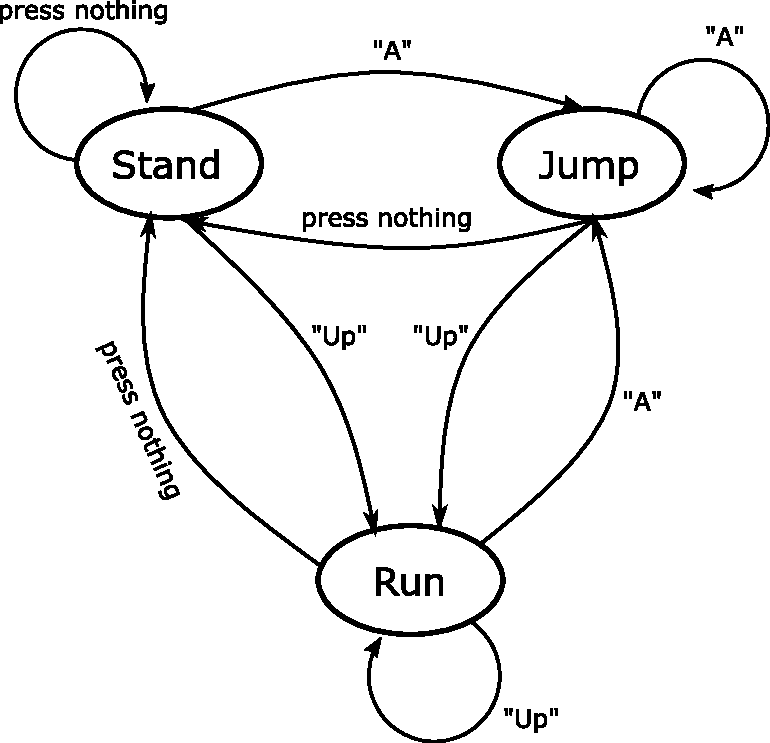
\includegraphics[scale=0.5]{files/Finite.pdf}
          \caption{Finite state machine for a video game character controlled by the player  \cite{brilliantFinite}.}
          \label{img:finite}
      \end{figure}

	\subsection{Markov Chains}
	A Markov Chain is a mathematical representation of a system that can pass from one state to another according to some defined probabilities to this transitions. The main characteristic of a Markov Chain is that the possible future states are independent from the initial state of the process. The set of possible states can be anything, depending on the problem at hand; for example, the states set can be letters, numbers, actions, etc. Figure \ref{img:markov} shows an example of a four-state chain for numbers.
    \begin{figure}[H]
        \centering
        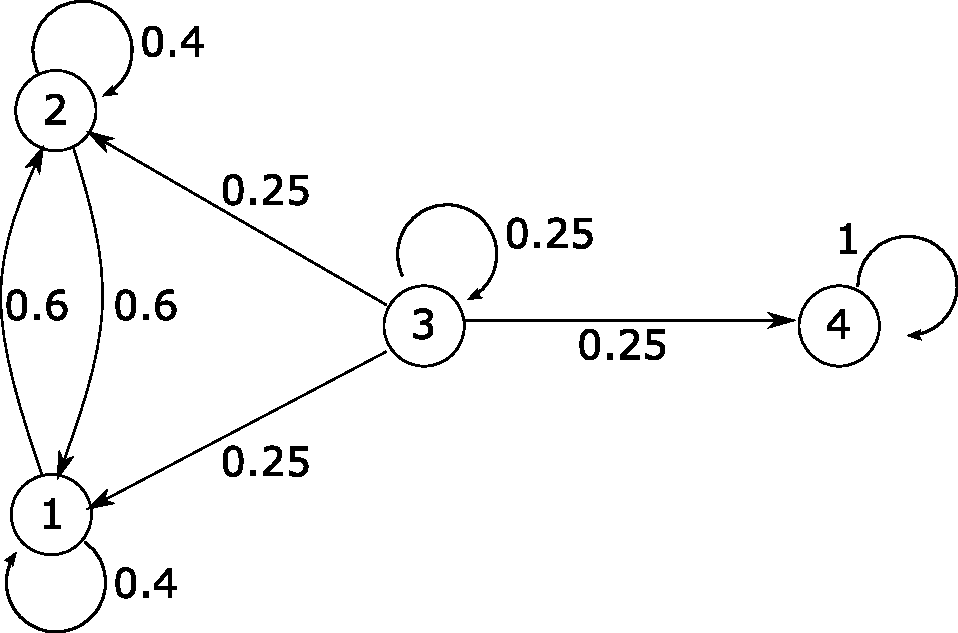
\includegraphics[scale=0.45]{files/Markov.pdf}
        \caption{Four-state Markov Chain \cite{brilliantMarkov}.}
        \label{img:markov}
    \end{figure}
    It is important to note that Markov chains follow the Markov property, which states: \textit{``The probability of future actions are not dependent upon the steps that led up to the present state''} \cite{brilliantMarkov}. Let $S=\{i_1$, $i_2$, $...$, $i_n\}$ be the set of possible states, a Markov Chain can be defined as sequence of random variables $X_1$, $X_2$, $X_3$, $...$ such that
    \begin{equation}
    	\forall n\in \mathbb{Z^+}, \quad P(X_n = i_n \mid X_0 = i_0, \, X_1 = i_1, \, \dots, \, X_{n-1} = i_{n-1}) = P(X_n = i_n \mid X_{n-1} = i_{n-1}),\quad i_k\in S
    \end{equation}

  \subsection{Bayesian Analysis}
    Bayesian Analysis can be defined as a set of practical methods for making inferences from data using probability models for quantities we observe and about which we wish to learn \cite{gelman2013bayesian}. The Bayesian Analysis is another approach to data analysis, just like Frequentist Analysis. Both approaches have their advantages, even though they do not share a similar methodology.
  \subsubsection{Bayesian vs. Frequentist}
  	\textbf{Frequentist}\\ The data to be analyzed is a result from random processes, therefore the data will change each time it is collected. The probability analyzed is
	\begin{equation*}
		P(y\mid\theta)
	\end{equation*}
    where $y$ is the known dataset and $\theta$ are parameters that were used to generate the random dataset. The problem to address by Frequentist Analysis is creating estimators in order to assign values to $\theta$. One big difference between Bayesian and Frequentist is that the second one has to create an estimator for each problem, while the Bayesian only uses one estimator: Bayes Formula.\\
    \textbf{Bayesian}\\ The opposite is considered: data is not random once it has been collected. The parameters, on the other hand, are considered random and a probability distribution is used to model its uncertainty, in other words, to model how much we know about an specific parameter. The probability analyzed is
    \begin{equation*}
    	P(\theta\mid y)
    \end{equation*}
    where $y$ is fixed, $\theta$ is fixed, but the knowledge about it will change. This is often addressed as ``inverse probability'', since you have a set of effects (often is the dataset) and you want to infer the causes. The Bayesian model is useful and flexible, it can be applied to a wide variety of problems; another advantage is that everything is addressed as a probability and, since people often have an intuitive idea of probabilities, the model and the results can be easy to interpret by almost everyone \cite{youtube1}.

  \subsubsection{Steps for a Bayesian Probability Model}
  According to Gelman \cite{gelman2013bayesian}, there are three general steps in order to build a Bayesian model, these are:
    \begin{enumerate}
    \item \textbf{Specify a Probability Model:} Build a model that includes everything that is influential and that you are interested to learn about.
    \item \textbf{Calculate a Posterior Distribution:} The posterior distribution $P(\theta\mid y)$ is referred as posterior because it tells us what we know about the unknown $\theta$ after having observed $y$. It is a function of the probability model we specified in last step. The difficulty in calculating the posterior distribution is the main reason why the adoption of Bayesian Analysis is poor. It is hard to calculate it analytically. But, if you manage to calculate the posterior distribution, you can get:
    \begin{multicols}{2}
    \begin{itemize}
    \item Point estimates
    \item Credible Intervals
    \item Quantiles
    \item Predictions
    \end{itemize}
    \end{multicols}
    \item \textbf{Check your Model:} As everything is represented with the model, is crucial its revision and check. Questions like: does the model fit the data? Are the conclusions reasonable? Are the outputs sensible to changes in the model structure?, can help determine whether the model is working properly or something needs to be rearranged \cite{youtube1}.
    \end{enumerate}

    \subsubsection{Bayes Formula}
    	As it was said before, Bayesian Analysis only uses one estimator: Bayes Formula. This formula was proposed by Thomas Bayes as follows \cite{youtube1}:
        \begin{equation}
        	P(\theta\mid y)=\frac{P(y\mid\theta)P(\theta)}{P(y)}
        \end{equation}
        Where
        \begin{itemize}
        	\item $P(\theta\mid y)$ is the posterior distribution.
            \item $P(\theta)$ is called the Prior, this is what we know about the unknown quantity before observing the data. This is the information state of parameters and it can be used to include information from previous studies, hence, the name Prior.
            \item $P(y\mid\theta)$ is called likelihood distribution. This is the representation of the observed data and it is used to update the prior distribution to posterior distribution. This distribution is closely related to a probability density function. This distribution holds a dataset $y$ constant and looks up which parameter $\theta$ is more likely to have generated that dataset.
            \item $P(y)$ is a normalizing factor, it can be calculated through the law of total probability as follows (depending on the type of data we are working on):
			\begin{equation}
				\begin{split}
               P(y)&=\sum_iP(y\mid\theta_i) P(\theta_i)\\
                    	&=\int P(y\mid\theta)P(\theta)d\theta
				\end{split}
			\end{equation}
        \end{itemize}

\subsubsection{Bayesian Inference in Video Games}
When applying bayesian inference in video games, it is a little different to the formal definition for making it useful in this context. First of all, the data prior to the observation will be the state that the variables that determine the behavior of the player; in this manner, this $y$ is considered as all the values that this variables have at some time $t$. On the other hand, the $\theta$ is represented by the state of another variable at a instant of time forward to the measure before. Likewise, the prior distribution just represents how likely is that the variables we are measuring have some arbitrary state. This is important to highlight, because this method of inference can allows us to infer the position of a object with respect to some measures before, in which state a character is and so forth. Generally, the discrete uniform distribution is used in this types of context due to the fact that most variables in video games take some finite set of values and, are equally likely that the variables takes those values \cite{coue2003using}.

Therefore, this type of inference is different in respect to other applications you might find but still does everything the other ones do.
